% +--------------------------------------------------------------------+
% | Sample Chapter 4
% +--------------------------------------------------------------------+

\cleardoublepage

% +--------------------------------------------------------------------+
% | Replace "This is Chapter 4" below with the title of your chapter.
% | LaTeX will automatically number the chapters.
% +--------------------------------------------------------------------+

\chapter{Implementación}
\label{makereference4}
A continuación, comenzaremos a exponer cómo hemos implementado nuestra aplicación, desde la arquitectura que hemos seguido, las tecnologías usadas para la parte 
\textbf{frontend} y la parte \textbf{backend} junto a las dificultades que nos hemos encontrado mientras trabajábamos y finalmente hablaremos de las herramientas de trabajo
utilizadas para facilitarnos el trabajo en equipo.
\section{Arquitectura}
\label{makereference4.1}
En cuanto a la arquitectura usada en nuestra aplicación hemos adjuntado un esquema que podemos observar en la figura 4.1. Nuestro cliente estará implementado tanto en \textbf{Android}
como en \textbf{Unity}, la aplicación general está en \textbf{Android}, mientras que la parte de realidad aumentada está desarrollada en \textbf{Unity} y usa \textbf{Vuforia}. Para el reconocimiento
de imágenes con \textbf{Vuforia} usamos un \textbf{Cloud} gratuito que nos ofrece para almacenar las imágenes ya que, tener todas las imágenes en la misma aplicación la cargaría de un peso innecesario.
Para la parte del servidor, hemos realizado una \textbf{API Rest} con \textbf{Spring}, usando además una base de datos relacional en \textbf{PostgreSQL}. 
\begin{figure}[H]
    \centering
    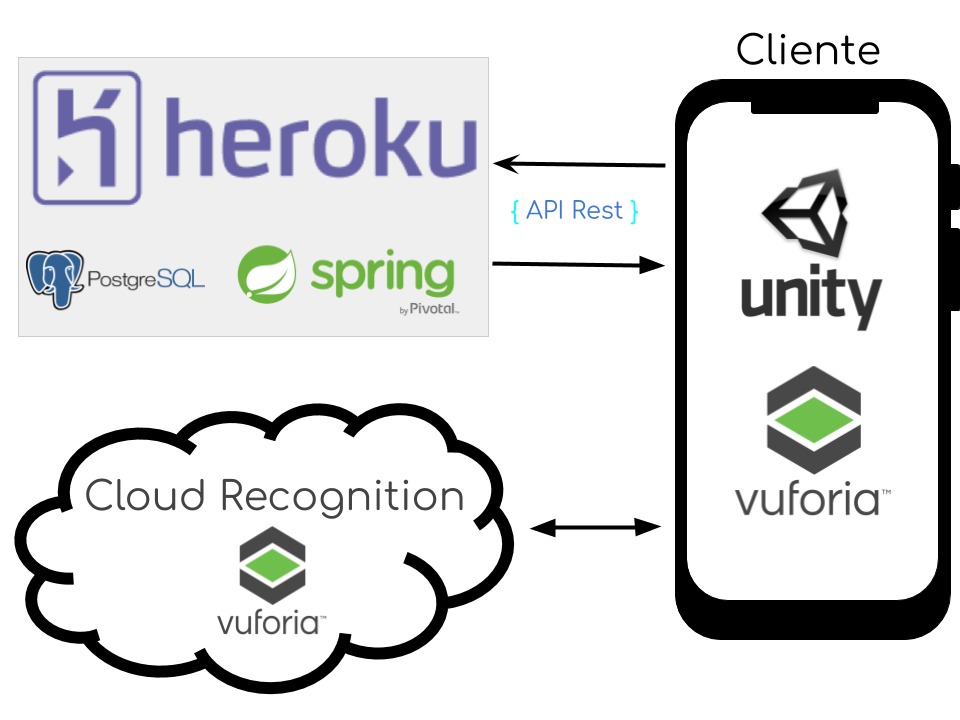
\includegraphics[width=6in]{figures/Arquitectura.png}
    \caption{Arquitectura}
\end{figure}
\section{Servidor}
\label{makereference4.2}
Nuestro servidor está programado en \textbf{Java}, usando el framework \textbf{Spring} para la creación de una \textbf{API Rest} que mediante peticiones \textbf{HTTP} y una base de datos relacional en \textbf{PostgreSQL} nos proporcionará
toda la información necesaria para alimentar de datos a nuestro cliente. El servidor necesita ser desplegado para que la aplicación pueda tener un uso real por lo que conseguimos desplegarlo de forma gratuita en \textbf{Heroku}, que además ofrece
facilidades para desplegar un servidor creado mediante \textbf{Spring}, por lo que nos facilitó el trabajo considerablemente.

\section{Aplicación}
\label{makereference4.3}
Nuestra aplicación está implementada principalmente en \textbf{Android}, las interfaces principales para el uso de los planes, recomendaciones y acceso a la información de las películas guardadas han sido desarrolladas mediante \textbf{Android Studio}. Sin embargo,
la parte del cliente que otorga el gran valor a nuestra aplicación está desarrollada en \textbf{Unity} y el uso de \textbf{Vuforia}, todas las escenas que aparecen al reconocer carteles de películas e imágenes de usuarios fueron implementadas de esta forma. \textbf{Vuforia} además nos ofrece un
servicio de \textbf{Cloud} para el almacenamiento de imágenes, a las cuales les asocia una valoración según lo fácil que le resultará a la aplicación reconocerla y un identificador único (\textbf{UUID}), que es el que usaremos para guardar la distinta información de dicha película o usuario en la base de datos.
La parte de la aplicación realizada en \textbf{Unity}, utiliza una serie de clases de la parte desarrollada en \textbf{Android} para realizar las peticiones al servidor y así poder mostrar información específica cuando se reconoce una cierta imagen.
Al principio hicimos que las dos partes realizaran las peticiones en sus respectivos lenguajes, pero decidimos que sería mejor que el acceso a la capa de datos se realizara por el mismo sitio y así conseguir que las distintas capas estuvieran separadas.
Además, las imágenes que mostramos en la parte de \textbf{Android} se almacenan en \textbf{Google Drive} y mediante la librería de \textbf{Picasso} las obtenemos en tiempo de ejecución, esto se ha implementado de esta forma por la misma razón por la que tenemos las imágenes a reconocer en un \textbf{Cloud}.

\section{Dificultades encontradas}
\label{makereference4.4}
A continuación, mostraremos una lista de todas las dificultades encontradas a la hora de implementar nuestra aplicación:
\begin{itemize}
    \item Desconocimiento del entorno de desarrollo y peculiaridades del desarrollo de aplicaciones en \textbf{Android}.
    \item Incompatibilidad de realización de peticiones \textbf{HTTP} en ciertas versiones de \textbf{Android}.
    \item Problemas a la hora de intentar desplegar el servidor de forma correcta para que fuera accesible siempre.
    \item Poca familiaridad con el uso de \textbf{Unity} y el lenguaje \textbf{CSharp********} para realizar la parte de realidad aumentada.
    \item Caducidad de las licencias gratuitas para el uso del \textbf{Cloud} de \textbf{Vuforia}.
    \item Primera vez usando el framework de \textbf{Spring} para la realización de una \textbf{API Rest}.
    \item Comunicación entre la parte cliente en \textbf{Android} y el servidor.
    \item Comunicación entre la parte cliente en \textbf{Unity} con la parte cliente en \textbf{Android}.
    \item Rendimiento en cuanto al reconocimiento de ciertas imágenes, sobre todo de personas, debido a la calidad de las mismas. El \textbf{Cloud} de \textbf{Vuforia} no las reconoce tan fácilmente como las de carteles de películas.
    \item Almacenamiento de imágenes en \textbf{Google Drive} y su obtención desde \textbf{Android} y \textbf{Unity}
\end{itemize}
\section{Herramientas de trabajo}
\label{makereference4.5}
Las distintas herramientas de trabajo que hemos decidido usar para que el trabajo realizado fuera más eficiente son las siguientes:
\begin{itemize}
    \item \textbf{Telegram}
    \item \textbf{Slack}
    \item \textbf{Trello}
    \item \textbf{GitHub}
\end{itemize}
